\documentclass[tikz,border=10pt]{standalone}
\usepackage{amsmath}
\usepackage{amssymb}
\definecolor{mantis}{RGB}{0, 105, 62}
\begin{document}
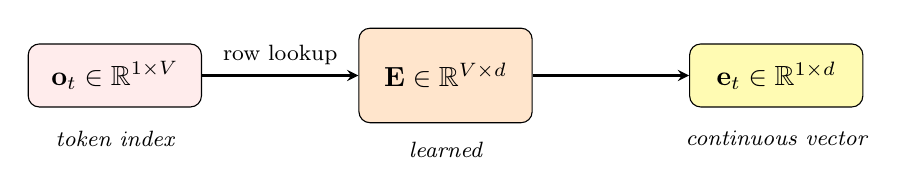
\begin{tikzpicture}[>=stealth]
    \node[draw, rounded corners, fill=pink!30, minimum width=2.2cm, minimum height=0.8cm] (onehot) at (0,0) {$\mathbf{o}_t \in \mathbb{R}^{1 \times V}$};
    \node[draw, rounded corners, fill=orange!20, minimum width=2.2cm, minimum height=1.2cm] (E) at (4.2,0) {$\mathbf{E} \in \mathbb{R}^{V \times d}$};
    \node[draw, rounded corners, fill=yellow!30, minimum width=2.2cm, minimum height=0.8cm] (emb) at (8.4,0) {$\mathbf{e}_t \in \mathbb{R}^{1 \times d}$};
    \draw[->, thick] (onehot) -- (E) node[midway, above, font=\footnotesize] {row lookup};
    \draw[->, thick] (E) -- (emb);
    \node[font=\footnotesize\itshape] at (0,-0.8) {token index};
    \node[font=\footnotesize\itshape] at (4.2,-0.95) {learned};
    \node[font=\footnotesize\itshape] at (8.4,-0.8) {continuous vector};
\end{tikzpicture}
\end{document}
